%!TEX root = ../thesis.tex
%*******************************************************************************
%****************************** Second Chapter *********************************
%*******************************************************************************

\chapter{Background}
\label{chapter background}

\ifpdf
    \graphicspath{{Chapter2/Figs/Raster/}{Chapter2/Figs/PDF/}{Chapter2/Figs/}}
\else
    \graphicspath{{Chapter2/Figs/Vector/}{Chapter2/Figs/}}
\fi

Measuring the blood flow of extremities provides the clinical community with valuable information about the overall health of a patient. Estimating immediate changes of blood volume within a limb offers insightful data on the wellness of "highways" that transport oxygen and nutrient to these tissues via the vasculature. Some diseases are attributed to problems in the micro or macro-vasculature. For instance, some of the disorders may include cardiovascular disease, peripheral vascular disease, diabetes and Raynaud's syndrome. In the absence of adequate blood supply, these tissues are liable to become ischaemic (\textit{isch} in Greek means to stop or block, which \textit{emia} implies blood flow).  If severely compromised, it can even lead to necrosis (death of tissue). In medicine, the clinician always attempts to salvage tissue whenever possible. Therefore, measuring the progression of disease or acute problems with the vasculature (in the extremities) can help clinicians decide on the optimal line of treatment, which may include a bypass graft or in extreme cases, amputation.

This chapter presents all the biological terminologies used in the entire document. The information provided here may be used as a reference when naming specific parts of the body. It will first cover the fundamentals of the circulatory system and blood. Subsequently, the anatomy of the upper limb will be described in detail along with the specific parts where the measurements will take place. Thereafter, the problems attributed to the lack of delivery of nutrients will be shown by providing an overview of the complications caused by bad blood delivery. Finally, since one of the objectives is to measure changes in blood flow in home settings, different instruments meeting this criterion will be described.   

\section{Circulatory system} %section 2.1
\label{section literature circulatory system}
The human body entails a closed circulatory system where the blood is enclosed within the blood vessels. It gets transported to and from the heart which works as a pump. The primary function of the circulatory system is to carry oxygen and nutrients to all the cells within the body and collecting the by-product of the entire metabolic process. Blood flows through the vessels that form a complex, elastic tubular network which reaches all cells of the body. The arteries are capable of carrying oxygenated blood, whereas the veins return de-oxygenated blood \cite{nichols2011mcdonald}. 

Blood is transported from the arterial to venous circulation within the capillaries. Meanwhile plasma passes through capillaries that are only about a cell's thickness in diameter. Subsequently, an increase of blood pressure expels interstitial fluid out of the capillary walls. In the end, some part of this fluid returns to the capillaries, with the rest flowing into lymphatic vessels. The different components of the circulatory system will be described in greater detail in the following sections. In particular, the anatomy of the arm will be elaborated upon since it is the part that will be tested by the new device \cite{Hall:2015aa}.

\subsection{The blood}
\label{section literature blood}
Blood is the main carrier of nutrients that pass through humans and vertebrate animals. It plays a significant role in strengthening the body's defence mechanism in order to combat infections. In short, it is in charge of transporting oxygen and collecting carbon dioxide from all the tissues that constitute the body. Blood requires different paths to be circulated in the human body; the circulatory system carries oxygenated and deoxygenated blood, also known as arterial and venous blood, respectively. The human body also uses arteries to transport oxygenated blood flowing from the heart through the lungs. Meanwhile veins are used to return deoxygenated blood into the heart and back to the lungs \cite{Hall:2015aa}.

\subsubsection{The blood plasma}
Notably, the blood plasma is one of the main electrical conductors in the human body. It is the suspending medium where the blood cells described by table \ref{table:cell} traverse throughout the body. Indeed, the extracellular fluids originate from the plasma's fluid.

Plasma gives the liquid properties to blood, since \SI{91}{\percent} of it is water \cite{scanlon2014essentials}. The solutes inside the plasma also assume pivotal roles at a cellular level. Within it, amino acids, glucose and vitamins are dissolved and are subsequently utilised by the cellular metabolic process. Additionally, there are hormones that regulate the activity of blood cells; their activation also results in the formation of chemical by-products within the circulature, such as nitrogen ($N$) and $CO_2$ \cite{Hall:2015aa, scanlon2014essentials}.

The plasma primarily comprises of salt and water. In fact, it is quite similar to seawater, albeit with a lower concentration of ions. Some of the ions present in significant numbers include sodium ($Na$), chloride ($Cl^-$) and bicarbonate ($HCO_3^-$) ions. However, traces of calcium, magnesium, copper, potassium and zinc are also found \cite{Hall:2015aa}.

Proteins, which are produced by the liver, are an essential component of the plasma. The most common protein found within it is albumin, which serves as depot protein and transport protein. For instance, it binds with long-chain fatty acids and bilirubin \cite{kragh1981molecular}. In addition, there are alpha and beta globulins that convey lipids, steroid hormones, and \textit{fibrinogen} used in the clotting process.

\subsubsection{Blood cells}
There are well known and identifiable components in blood. Approximately half of its volume is made up of plasma, the properties of which were described previously. The remaining half   comprises of red blood cells (erythrocytes), white blood cells (leukocytes or monocytes) and platelets (thrombocytes)\cite{scanlon2014essentials}. In summation, the primary function of red blood cells is to transport oxygen; the white blood cells meanwhile are in charge of the immunological response, and platelets, the clotting process \cite{Hall:2015aa}.

However, these cells also perform other specialised tasks. Their properties and characteristics are described in greater detail in table \ref{table:cell}; it also includes cells quantity per microliter (\si{\micro\litre}) of the human blood. Importantly, there are diverse specialised subtypes of white cells and platelets as well, but they are beyond the scope of the existing study \cite{Hall:2015aa}.

\begin{table}
	\caption[Blood cell classification]{Blood cell classification}
	\label{table:cell}
	\centering
	\begin{tabular}{ >{\raggedright}p{0.18\textwidth}  
			>{\raggedright}p{0.12\textwidth} 
			p{0.22\textwidth} 
			p{0.37\textwidth}}
		\toprule
		\textbf{Cell Type }
		& \textbf{Quantity} 
		& \textbf{Geometry} 
		& \textbf{Characteristic} \\
		\midrule
		Red Blood Cells (RBCs) or erythrocytes 
		& \numrange{5e6}{6e6} 
		& Shape: Disk \newline Diameter: 6-\SI{8}{\micro\meter} \newline Thickness: \SI{2}{\micro\meter} 
		& \begin{tabular}[t]{P{0.34\textwidth}} 
			\tabitem Principal medium to deliver oxygen \\
			\tabitem Lack of nucleus \\
			\tabitem Cytoplasm rich in negatively charged Iron-containing Hb \\
			\tabitem Contains Ions of Sodium ($Na^+$) and Potassium ($K^+$) \\
			\tabitem Typical bilayer lipid membrane (Lipid composition defies physical properties such as membrane permeability and fluidity) 
		\end{tabular} \\
		\midrule
		White Blood Cells (WBC) or Monocytes 
		& \numrange{4e3}{11e3} 
		& Shape: Irregular \newline Diameter: 10-\SI{20}{\micro\meter} \newline Monocytes: 14-17 
		& \begin{tabular}[t]{P{0.34\textwidth}} 
			\tabitem Composed five different type of specialised cells to target different illnesses\\
			\tabitem Make part of the immune system \\
			\tabitem High count of these cells are indicators of disease 
		\end{tabular} \\
		\midrule
		Platelets 
		& \numrange{150e3}{400e3} 
		& Shape: Irregular \newline Diameter: 2-\SI{3}{\micro\meter}  
		& \begin{tabular}[t]{P{0.34\textwidth}}
			\tabitem Lack of nucleus  \\
			\tabitem Responsible for procoauglant activity \\
			\tabitem If count to low excessive blood may occur. Too high blood cloth might form (thrombosis)
		\end{tabular} \\ 
		\bottomrule
	\end{tabular}
\end{table}

\subsection{Blood vessels}
The blood leaves the heart through arteries that reach all organs of the body. This network of arteries branches into a microscopic size, at which point, they are referred to as arterioles. From this point onwards, blood enters the capillaries, which are essentially tiny thin-walled tubes that attain the size of a cell. Venules collect the blood flowing out of the capillaries before moving on to the main veins, which then carry it back to the heart \cite{Hall:2015aa}.

Arteries, arterioles, veins and venules are composed of the same cellular structure (see figures \ref{fig:arteries composition} and \ref{fig:veins composition}). The innermost part of these vessels is an epithelial coating referred to as the endothelium. A thin layer of elastic fibres, a smooth muscle and connective tissue engulf the endothelium. Capillaries are much thinner than these vessels. Indeed, capillaries are comprised only of endothelium cells, which facilitate the exchange of fluids between the blood and the surrounding tissue (see figure \ref{fig:capillaries composition}). This interchange of molecules and ions between both occurs by diffusion, filtration at the capillary walls, and transport through endothelial cells \cite{Hall:2015aa}. Hence, this is here where the exchange of gases and metabolites occurs between the blood and the body's cells \cite{johnson2001biology}.

\begin{figure*}[!htbp]
	\centering
	\begin{subfigure}[t]{0.33\textwidth}
		\centering
		\includegraphics[width=5cm]{figure1a}
		\caption{Layers of the arteries}
		\label{fig:arteries composition}
	\end{subfigure}%
	~ 
	\begin{subfigure}[t]{0.33\textwidth}
		\centering
		\includegraphics[width=5cm]{figure1c}
		\caption{Layers of the venous}
		\label{fig:veins composition}
	\end{subfigure}
	~ 
	\begin{subfigure}[t]{0.33\textwidth}
		\centering
		\includegraphics[width=5cm, trim={0 0 2cm 0},clip]{figure1b}
		\caption{Layers of the capillaries}
		\label{fig:capillaries composition}
	\end{subfigure}
	\caption[Layers of the blood vessels]{The arteries and veins involve the same kind of layers. However, the smooth muscle is thicker in arteries as compared to the veins. The capillaries have a thin wall and are composed only of endothelium. Figure adapted from \cite{johnson2001biology}.}
	\label{fig:vessels composition}
\end{figure*}

\subsubsection{Arteries and arterioles}
The arteries slightly differ from the arterioles in their composition. The main arteries contain additional elastic fibres within them, thus enabling greater compliance while receiving blood coming out the heart. On the other hand, smaller arteries and arterioles contain a thicker smooth muscle layer in their tunica media which allows them to resist bursting \cite{Hall:2015aa, scanlon2014essentials}.  

There is a direct relation between the diameter of the vessel and the frictional resistance to blood flow. The resistance to blood flow is inversely proportional to the radius of the vessel. Halving the diameter of a blood vessel increases its frictional resistance by 16 times. Hence, the greatest resistance to blood flow in this branch of the circulatory system occurs in small arteries and arterioles \cite{Hall:2015aa}. Moreover, when there is a contraction of the smooth muscle layer of arterioles, it leads to vasoconstriction, which increases resistance and decreases blood flow. On the other hand, upon the relaxation of this muscle, vasodilation occurs, thus reducing resistance and increasing blood flow. Local chemical factors, the sympathetic system or even the hormones can control both muscle activities. Furthermore, blood flow towards some organs can be regulated by precapillary sphincters. These rings of smooth muscle are capable of shutting down capillary beds in totality. For instance, in cold weather, these precapillary sphincters may close to contribute to the vasoconstriction, thereby limiting heat loss \cite{Hall:2015aa, scanlon2014essentials}.  

\subsubsection{Capillaries}
As described before, capillaries are considerably smaller than the rest of the blood vessels. On average, each one of them is about \SI{1}{\milli\meter} long, \SI{8}{\um} diameter, and \SI{0.5}{\um} thick, which is just about sufficient to allow a single red blood cell (RBC) (\SIrange{4}{9}{\um}) to pass through them. The capillary tree is so dense and extensive that every cell in the human body is within \SI{100}{\um} of reach.  Due to the sheer enormity (in terms of numbers) and the intricacy of their numbers, they have the greatest cross-sectional area of any other kind of blood vessel. Therefore, the blood decreases its velocity, allowing more time to exchange metabolites with the surrounding extracellular fluid. As soon as the blood leaves the capillary, the exchange of $O_2$, nutrients, $CO_2$ and waste products occurs \cite{Hall:2015aa, scanlon2014essentials}. 

Notably, the heart must produce enough pressure to be able to overcome the resistance of the blood passing the arterial tree into the capillaries. However, blood loses most of its pressure when moving through the capillary network and also by entering to the veins. 

\subsubsection{Venules and veins}
Venules collect the blood flowing out of the capillaries which is then deposited in the larger veins that leads the blood back to the heart. Due to the pressure in the venous return being one-tenth that of the arteries, venules and veins comprise of a thinner layer of smooth muscle. This pressure gradient also helps the blood pass through the narrow passages of the capillaries. Most of the blood volume is contained within the veins, which also have the ability of expansion in order to increase the body's blood capacity, if needed. In order to enable the blood to return from the extremities, the surrounding skeletal muscle contracts by compressing the veins and pushing the blood back into the heart\cite{Hall:2015aa, scanlon2014essentials}. Additionally, the veins contain valves that only blood to flow in only one direction. However, a failure of any of these valves may trigger vascular problems, such as varicose veins. 

\begin{figure}[!htpb]
	\centering
	\includegraphics[width=0.5\textwidth,keepaspectratio]{figure2}    
	\caption[Venous return through skeletal muscle]{The vein only flows in on direction helped by valves along the vessel. Skeletal muscle contraction aids the return of blood to the heart. Figure adapted from \cite{johnson2001biology}. }
	\label{fig:venous return}
\end{figure}

\section{Cardiac cycle}
\label{background cardiac cycle}
It is important to understand how the heart operates because changes in volume are synchronous to the heart beat. As part of the circulatory cycle, the heart needs to overcome the pressure of pushing RBC's through the capillaries. Hence, the heart is required to work as a dual pump, pushing out arterial and collecting venous blood. The cardiac cycle is a periodic task that begins at the beginning of one heart beat until the commencement of the following one. The cycle is divided into ventricular contraction and ventricular relaxation known as systole and diastole, respectively \cite{Weinhaus2015}. 

Each cardiac cycle is subdivided into phases where the heart experiences intense pressure change at a constant volume, or a volume change with a minor alteration in pressure. During the systolic cycle, the heart experiences (1) isovolumetric contraction followed by (2) blood ejection. On the other hand, diastole cycle entails the following steps (1) isovolumetric relaxation, (2) early diastolic filling,(3) slow ventricular filling (diastasis) and (4) atrial filling \cite{fukuta2008cardiac}. The heart rate is inversely proportional to the cardiac cycle and changes in accordance to the body's needs. An average heart rate is close to 75 beats per minute, wherein a single beat lasts around \SI{0.8}{\second} \cite{Hall:2015aa}.

At rest, the duration of the systolic cycle takes about 1/3 of the total heart cycle, with the rest being accounted for by the diastolic cycle. In case of a high heart rate, such as during exercise, this proportion changes; the duration of diastole takes much less time as compared to systole. The following sections will describe the changes occurring in the heart, in addition to the pressures, electrical activity and heart sounds along each cycle \cite{Hall:2015aa}.

\begin{figure}[!htpb]
	\centering
	\includegraphics[width=8.5cm,keepaspectratio]{figure_pressure}    
	\caption[Changes of Pressure and Volume in the heart - ECG]{Pressures, volume changes and ECG changes during one heart cycle. During the systolic cycle, the heart experiences (1) isovolumetric contraction followed by (2) blood ejection. On the other hand, diastole cycle entails the following steps (1) isovolumetric relaxation, (2) early diastolic filling,(3) slow ventricular filling (diastasis) and (4) atrial filling \cite{fukuta2008cardiac}}
	\label{fig:heart cycle}
\end{figure}

\subsection{Systole}
\subsubsection{Isovolumic (Isometric) contraction}
The etymology of the word isovolumic comes from ancient Greek, the prefix \textit{isos} meaning equal and \textit{volumetric} to reference volume. Hence, the heart keeps the same blood volume in this cycle, while the ventricles contract \cite{Hall:2015aa}.

\begin{figure}[!htpb]
	\centering
	\includegraphics[height=4cm,keepaspectratio]{figure_3}   
	\caption[Heart during isovolumic (isometric) contaction]{Cross section of the heart during isovolumic (isometric) contraction. The contracted area is represented by the red colour.}
	\label{fig:heart isovolumic}
\end{figure}

Figure \ref{fig:heart cycle} illustrates the variation of pressure within the left ventricle, the right atrium, the aortic pressure and the ventricular volume. As the valves are shut, the ventricles are contracted and blood is unable to leave from the heart, the ventricular pressure increases but causes no changes in the blood's volume. In the end, the total volume inside the ventricles is equivalent to the end-diastolic volume (about \SI{130}{\milli\litre} \cite{fukuta2008cardiac}. In the atria, owing to the differential of pressure between chambers, the atrioventricular ends up bulging backwards. Therefore, this valve change causes a small pressure variation in the right atrium. It is depicted as point c in the same figure. The pressure in the systemic and pulmonary arteries drops at a constant rate \cite{Hall:2015aa}. 

The electrocardiogram waveform illustrated in figure \ref{fig:heart cycle} displays the electrical activity of the heart during this section of the cycle. In short, the depolarization of the heart begins from the atrioventricular node that spreads through the bundle of His and Purkinje fibres into the septum and the walls of both ventricles. This in turn causes the QRS complex, as shown in the same figure. Simultaneously, the atrial repolarisation causes the atrial T wave which remains invisible in the ECG because the QRS complex covers it.

\rvmynote{Add a reference to this text from a medical book.}

\subsubsection{Ejection}
During this cycle, the mechanics of the heart experiences the following changes. The gradient of pressure is greater in the left ventricle as compared to the aorta. The pressure of the right ventricle exceeds that of the pulmonary artery, causing the semilunar valves to open. Due to the ventricular contraction, the blood is ejected from both ventricles to the aorta; in addition, the pulmonary arteries and atrioventricular valves are closed \cite{Hall:2015aa}.

\begin{figure}[!htpb]
	\centering
	\includegraphics[height=4cm,keepaspectratio]{figure_6}
	\caption[Cross section of the heart during the ejection cycle]{Cross section of the heart during the ejection cycle. The contracted area is denoted by red colour. The semilunar valves are open.}
	\label{fig:heart ejection}
\end{figure}

This cycle divides itself into a rapid and slow ejection. The increasing ventricular pressure during the contraction creates the sudden purge of blood toward the arteries. Then, the blood volume within the ventricles and arteries begins to drop. Due to the pressure difference between the two, the blood gets ejected slowly. During this cycle, the maximum pressure of the left ventricle generally reaches about \SI{120}{\mmHg}, which is known as systolic pressure and \SI{25}{\mmHg} in the right ventricle. These pressures also get transferred to the aorta and pulmonary arteries, respectively which also begin to drop after reaching these peaks. In terms of blood volume, under normal conditions while resting only, \SI{70}{\milli\litre} the ejection of blood occurs, which is known as stroke or systolic volume. The rest \SI{60}{\milli\litre} remains in the heart until the end of the cycle, known as end-systolic volume. The relationship between stroke volume and the end-diastolic volume is known as ejection fraction, which \SI{60}{\percent} lies in the normal physiological range. The atria also contracts during this cycle. The pressure in the atria and main vein vessels decreases because they are elongated by the shortening of the ventricles, thereby causing a drop in the atria's pressure. 

From the electrical standpoint, the ventricles are completely depolarised at the beginning of this cycle, which is equivalent to the ST segment of the electrocardiogram. Due to ventricular repolarisation, the T wave can be seen during the second part of this stage. 

\subsection{Diastole}
\subsubsection{Isovolumic relaxation}
In the heart's mechanics, once the heart completes its systole, the ventricles relax, and the pressure begins to reduce rapidly. Due to blood inertia occurring for a short period, the blood flows out of the ventricles. The elevated pressure in the aorta and pulmonary arteries pushes back a little amount of blood towards the ventricle, which also leads to the closure of the semilunar valves. Additionally, the atrioventricular valves are closed because the pressure in the atria is lower than that of the ventricle \cite{Hall:2015aa}.

\begin{figure}[!htpb]
	\centering
	\includegraphics[height=4cm,keepaspectratio]{figure_9}
	\caption[Heart during isovolumetric relaxation cycle]{Cross section of the heart during the isovolumic relaxation cycle. Semilunar and atrioventricular valves are closed in this stage.}
	\label{fig:heart isovolumetric relaxation}
\end{figure}

The changes of pressures and volumes in the different chambers occur as follows. The ventricles relax rapidly, decreasing their pressure without altering the blood volume, which explains the name isovolumetric relaxation. Indeed, the blood remaining within the ventricle is still the end-systolic volume (\SI{60}{\milli\litre}. This relaxation period causes a great drop in ventricular pressure until it gets close to zero in both ventricles towards the end of this cycle. The atria are filled with blood from the veins, whereas the atrioventricular valves remain closed. This action begins to raise the pressure within the atria (v wave in the figure \ref{fig:heart cycle}). In the arteries, the decrease of pressure is interrupted by the dicrotic notch, which signifies a temporary increase in pressure that creates a blood backflow which also ends up closing the semilunar valves. 

During this period, the ventricle is completely repolarised, thereby completing the T wave in the ECG, as shown in the figure \ref{fig:heart cycle}.

\subsubsection{Rapid ventricular filling}
During this cycle, the ventricular pressure reaches a point where it becomes lower than the atrial one. Therefore, the atrioventricular valves open up, allowing the blood accumulated in the atria to pass quickly into the ventricles. Most of the ventricular filling occurs during this stage. Furthermore, the blood volume within the ventricle increases, but its pressure changes insignificantly towing to the muscle relaxation. In the atria, the decrease in pressure is caused by the blood that is expelled from the atria into the ventricles \cite{Hall:2015aa}. 

\begin{figure}[!htpb]
	\centering
	\includegraphics[height=4cm,keepaspectratio]{figure_12}
	\caption[Heart during rapid ventricular filling]{During rapid ventricular filling the atrioventricular valves open allowing blood to pass from the atria to the ventricles rapidly. The semilunar valves remain closed.}
	\label{fig:heart rapid ventricular filling}
\end{figure}

The semilunar valves remain closed during this stage, although the arterial pressure starts to decrease slowly. In the arteries, the blood pressure never reduces to zero as it does in the heart because of their recoil properties. Indeed, the minimum arterial pressure within the systemic circulation during a heart beat is commonly \SI{80}{\mmHg}, which is referred to as diastolic pressure. In contrast, in the pulmonary circulation, the pressure can decline up to \SI{8}{\mmHg}. The electrical activity of the heart remains null during this cycle. This explains the rationale of the isoelectric representation in the ECG wave.


\subsubsection{Slow ventricular filling}
In this stage, no change occurs in the mechanical activity of the heart. Certainly, the valves remain the same as is the case in a rapid ventricular cycle. The atrioventricular valves are open and the semilunars get closed. A small volume of blood flows into the ventricles from the veins passing the atria, filling up the ventricle slowly. The pressure in the ventricles still continues at zero, while the pressure in the atria increases slightly. Meanwhile, the pressure in systemic and pulmonary circulation declines at a constant rate \cite{Hall:2015aa}. 

In the heart's electrical path, the sinoatrial node depolarises at the end of the cycle and the electrical activity follows its course all around the heart, producing the p wave, as shown in the ECG plot. 

\subsubsection{Atrial systole}
Atrial systole denotes the last part of the cardiac cycle. In the mechanics of the heart during this phase, the ventricles fill up entirely, whereas the atrioventricular valves open and the semilunar valves end up closing. Additionally, an atrial contraction ejects blood from the atria to the ventricle \cite{Hall:2015aa}s. 

Thus, the atria eject approximately \SI{25}{\percent} of the ventricular filling volume into the ventricles. Subsequently, the ventricular myocardium relaxes, causing a slight change of pressure in the ventricles that remains close to zero. At the end of the atrial systole, the total blood volume within the ventricles at the end-diastolic volume is about \SI{130}{\mmHg}. Due to the atrial contraction, there is an increased pressure of these chambers; this can be seen as wave \textbf{a} in the venous pulse in figure \ref{fig:heart cycle}. Finally, the arteries' pressure continues to decline at a constant pace.

The P wave of the ECG trace in figure \ref{fig:heart cycle} represents the moment at which atrial depolarisation occurs. Subsequently, the depolarisation spreads from the atria into the atrioventricular node, which is portrayed by the PR segment in the ECG.

\begin{figure}[!htpb]
	\centering
	\includegraphics[height=4cm,keepaspectratio]{figure_17}
	\caption[Heart's chambers movement during Atrial systole]{Ventricular pressure continues almost in zero (red line). The arterial pressure continues to decrease slowly (black line), there is a rise in the atrial pressure (dark blue). The ventricles are completely full (light blue) to end-diastolic volume (\SI{130}{\milli\litre}).}
	\label{fig:heart atrial systole}
\end{figure}


\section{Upper limb anatomy}
\label{section literature anatomy}
The experimental work of this document described in chapter \ref{chapter procedure} was carried out in the forearm. This section elaborates on the anatomy of the upper arm and the forearm. This information helps convey the position of the electrodes as well as the nearby tissue that interacts with the impedance plethysmography device. 

The arm forms part of the upper limb of the human anatomy. It divides into three sections; the upper arm, the forearm and the hand. The upper arm and forearm will be explored in greater depth as this is what was involved in this study. The upper arm lies between the shoulder and the elbow and the forearm comprises of the portion between the elbow and the wrist. 


\subsection{Bones of the arm}
Figure \ref{fig:upper limb bones} shows the bones of the upper arm of which, the humerus form the only bone in this part of the arm. This bone connects the scapula to the radius and ulna, which comprise the bones of the forearm. These bones connect to the carpus bones in the hand that comprises the wrist. The rest of the bones are made up of the metacarpus and the phalanges. 

\begin{figure}[!htpb]
	\centering
	\includegraphics[width=0.4\textwidth,keepaspectratio]{figure_20} 
	\caption{Bones of the upper arm}
	\label{fig:upper limb bones}
\end{figure}


\subsection{Muscles of the arm}
The muscles of the arm are divided by fascial compartments called the lateral and intermuscular septa. This subsequently divides these muscles into anterior (see figure \ref{fig:upper arm anterior}) and posterior compartments (see figure \ref{fig:upper arm posterior}). The upper arm comprises of four muscles. Within the anterior compartment are the biceps brachii, brachialis and coracobrachialis, whereas the triceps brachii is in the posterior compartment \cite{scanlon2014essentials}. 

\begin{figure}[!htpb]
	\begin{subfigure}[t]{0.52\textwidth}
		\centering
		\includegraphics[height=5.5cm,keepaspectratio]{figure15a}
		\caption{Muscles of the anterior compartment}
		\label{fig:upper arm anterior}
	\end{subfigure}
	~
	\begin{subfigure}[t]{0.44\textwidth}
		\centering
		\includegraphics[height=5.5cm,keepaspectratio]{figure15b}
		\caption{Muscles of the posterior compartment}
		\label{fig:upper arm posterior}
	\end{subfigure}
	\caption{Muscles of the upper arm}
\end{figure}

The forearm comprises of many muscles that perform flexion and pronation of the wrist and fingers. The anterior compartment is divided into three: superficial, intermediate and deep. Within the superficial compartment are the flexor carpi ulnaris, palmaris longus, flexor carpi radialis and the pronator teres. The lone muscle of the intermediate compartment is the flexor digitorum superficialis \cite{scanlon2014essentials}. All these muscles are displayed in figure \ref{fig:forearm anterior}.

\begin{figure}[!htpb]
	\centering
	\includegraphics[height=4.5cm,keepaspectratio]{figure16}
	\caption{Muscles of the anterior compartment}
	\label{fig:forearm anterior}
\end{figure}	

Finally, as illustrated in figure \ref{fig:forearm deep} three muscles are located in the deep compartment: the flexor digitorum profundus, flexor pollicis longus and the pronator quadratus.

\begin{figure}[!htpb]
	\centering
	\includegraphics[height=4.5cm,keepaspectratio]{figure17}
	\caption{Muscles of the deep compartment}
	\label{fig:forearm deep}
\end{figure}

\subsection{Circulation of the arm}
\subsubsection{Arterial circulation}
The subclavian arteries located in the chest area supply the blood into the arm.  The right arm blood supply comes from the right subclavian artery, which is attached to the brachiocephalic trunk (see figure \ref{fig:subcalvian}). On the other hand the blood supply of the left arm is directly sourced from the subclavian artery connected to the arch of the aorta \cite{scanlon2014essentials}. 

\begin{figure}[!htpb]
	\centering
	\includegraphics[height=4.5cm,keepaspectratio]{figure18}
	\caption{Origin of the subclavian arteries}
	\label{fig:subcalvian}
\end{figure}

When these arteries pass through the axilla, they are known as axillary arteries. From this artery arise other arteries, such as the posterior and anterior circumflex arteries which supply blood into the shoulder section, as well as the subscapular artery which is the largest among them \cite{scanlon2014essentials}. 

Hereafter, as shown in figure \ref{fig:upper arm circulation} the axillary artery becomes the brachial artery at the teres major muscle, which supplies blood for the entire arm.  From this artery arise other arteries that supply blood to the tissues in the upper arm. These include the profunda brachii, which is the deep artery of the arm that traverses through the posterior surface of the humerus \cite{scanlon2014essentials}. 

\begin{figure}[!htpb]
	\centering
	\includegraphics[height=6cm,keepaspectratio]{figure19}
	\caption{Origin of the subclavian arteries}
	\label{fig:upper arm circulation}
\end{figure}

As seen in figure \ref{fig:forearm aretries}, as soon as the brachial artery passes through the cubital fossa (front of the elbow joint) underneath the brachialis muscle, this artery bifurcates, becoming the radial and ulnar arteries. The radial artery supplies blood into the posterior tissues of the arm along with the ulnar to the anterior. At the carpus bones, these arteries anastomose in the hand, forming deep and superficial palm arches that supply blood into the different tissues located in the hand \cite{scanlon2014essentials}. 

\begin{figure}[!htpb]
	\centering
	\includegraphics[height=4.5cm,keepaspectratio]{figure20}
	\caption{Forearm arteries}
	\label{fig:forearm aretries}
\end{figure}

\subsubsection{Venous circulation}
The veins of the arm are anatomically split into the superficial and deep veins (see figure \ref{fig:arm veind}). The biggest superficial veins within the upper limb are the cephalic and basilic veins. The latter originates at the venous branches of the hand, close to the teres major, at which point the vein goes deep into the arm. It is at this point that this vein combines with the brachial veins to form the axillary vein \cite{scanlon2014essentials}. 

The cephalic vein begins at the dorsal venous network of the hand. It ascends on the anterolateral region and passes to the anterior part of the limb at the elbow. In the same section, the median cubital vein connects the cephalic and basilic veins. At the axilla, the cephalic vein joins with the axillary vein \cite{scanlon2014essentials}. 

The deep fascia contains the deep veins within the upper limb. These veins are paired to either side of the brachial, radial and venous artery. Hence, they inherit the same names.  In fact, the pulsation of the brachial artery facilitates the venous return of the arm. This effect is referred to as vena comitantes. The perforating veins link the deep and superficial veins of the upper arm \cite{scanlon2014essentials}. 

\begin{figure}[!htpb]
	\centering
	\includegraphics[height=10cm,keepaspectratio]{figure21}
	\caption{Forearm arteries}
	\label{fig:arm veind}
\end{figure} 

\section{Oxygen transportation}
\label{section literature 1.2}
Oxygen ($O_2$) forms an essential component required by all cells of the body to complete the metabolic processes. This is transported by haemoglobin (Hb) that form part of the red blood cells (RBCs). Oxygen is required for the chemical reactions that eventually convert biochemical energy created by nutrients coming from food into cellular energy known as coenzyme or adenosine triphosphate (ATP). As a result of this reaction, a waste product is released from the cell. A human cell cannot survive without Oxygen for more than a few minutes~\cite{culmsee2005apoptosis}.

Inadequate oxygen supply into the bodily tissues is known as hypoxia. There are different classifications of hypoxia depending on its cause~\cite{marieb2007human} which are described as follows: 

\begin{enumerate}
	\item \textbf{Anaemic Hypoxia:} It is a condition wherein a body part or an organ suffers from poor $O_2$ delivery. Some of the causes include a small count of RBCs and abnormal or inadequate Hb levels.
	\item \textbf{Ischaemic (stagnant) hypoxia: }This is caused when blood circulation is reduced or blocked. Among the many causes, the most common include congestive heart failure that may cause body-wide hypoxia, emboli or thrombi, blocking oxygen supply to the tissue distal from the occlusion. 
	\item \textbf{Histotoxic hypoxia: }Mainly caused by metabolic poisoning such as the ingestion of cyanide. Here, the cell is unable to use $O_2$ for metabolic purposes, even though there is an appropriate amount of $O_2$ being delivered by the body.
	\item \textbf{Hypoxemic hypoxia:} It is denoted by a decrease in the arterial oxygen partial pressure ($PO_2$). Some of the causes include an imbalance in the ventilation-perfusion coupling mechanism, poor ventilation attributed to pulmonary disease and breathing air with a low $O_2$ content. Carbon monoxide ($CO$) poisoning is another major reason because it has \num{200} times more affinity with Hb than $O_2$. Thus, in scenarios that involve high concentrations of CO, such as fires, this could easily lead to death.
\end{enumerate}

\subsection{Problems derived from poor blood delivery} %Section 4,1
\label{section literature 4,1}
Now that some of the problems of poor oxygen transportation at a cellular level have been touched upon, let us understand, in greater detail, the illnesses caused due to poor or total lack of blood supply to human tissues, particularly human limbs. 

Ischaemia is a medical ailment that is attributed to insufficient supply of blood into an organ. For instance, if an artery blockage occurs, all the tissues below that blocked path will suffer from the starvation of oxygen and other critical nutrients. Different causes could cause the blockage of an artery; these can include internal or external factors. In specific reference to lower limbs, ischaemia signifies a major cause of disability, cardiovascular morbidity and mortality~\cite{novo1995patients}.

There are different diseases that compromise the functioning of limbs; this includes a peripheral arterial disease (PAD), of which, there are two subtypes. One of these is critical limb ischaemia (CLI), whereby the patient could lose their limb in the absence of timely medical intervention. One of the first symptoms is that the patient experiences continuous pain at the extremity, even at rest ~\cite{novo2004critical}. 

Clinically there are different methods to assess the development of this illness. Some scales of qualitative evaluation have been developed, such as the Rutherford classification, the Leriche-Fontaine classification, and the TACS II classification of femoral and popliteal lesions~\cite{norgren2007inter}. Health practitioners use a survey, which is an indicator of pain when walking and a visual inspection. This makes it possible to determine the stage or the severity of the arterial occlusion. 

Table \ref{table:Fontaine} illustrates the different stages of the Leriche-Fountaine classification along with the various steps that are considered to evaluate the illness.
As shown by this table, there are various levels of stratifying the severity of this disease in accordance to the symptoms related to pathophysiology. There are also different methods to examine the severity of this disease using imaging techniques.

\begin{table}
	\caption{Leriche-Fontaine classification}
	\centering
	\label{table:Fontaine}
	\begin{tabular}{p{1.8cm} >{\raggedright}p{3.6cm} p{3.4cm} p{4.8cm}}
		\toprule
		\textbf{Stages}& \textbf{Symptoms} & \textbf{Pathophysiology} & \textbf{Pathophysiological \newline classification} \\
		\midrule
		Stage I & Asymptomatic or effort pain & Relative hypoxia & Silent Arteriopathy \\
		\midrule
		Stage II A & Effort pain \newline Pain free walking distance > \SI{200}{\meter} & Relative hypoxia & Stabilized Arteriopathy \newline Non-Invalidant claudication \\ 
		\midrule
		Stage III A & Rest Pain \newline Ankle arterial pressure > \SI{50}{\mmHg} & Cutaneous hypoxia \newline Tissue acidosis \newline Ischemic neuritis & Instable arteriopathy \newline Invalidant claudication \\
		\midrule
		Stage III B & Rest pain \newline Ankle arterial pressure < \SI{50}{\mmHg} & Cutaneous hypoxia \newline Tissue acidosis \newline Ischemic neuritis & Instable arteriopathy \newline
		Invalidant claudication \\
		\midrule
		Stage IV & Trophic lesions \newline Necrosis or Gangrene & Cutaneous hypoxia \newline 
		Tissue acidosis & Necrosis \newline Evolutive arteriopathy \\
		\bottomrule
	\end{tabular}
\end{table}

There are a significant number of illnesses caused by the inadequate delivery of blood towards a limb. According to their physiology, they can be divided into a disease which either affects the microcirculation or main vessels, or both. The following is just an example of the different diseases that may necessitate continuous blood flow monitoring in acute or chronic settings.

\subsubsection{Peripheral vascular disease}
\label{section literature 2.1}
A disease which causes the reduction of blood towards a limb is known as peripheral vascular disease (PVD) or peripheral arterial disease (PAD). This illness is a progressive vascular condition caused by the blockage, narrowing, or spasms in a blood vessel (arteries, veins or lymphatic vessels), thereby, altering the blood circulation to and from upper or lower extremities.  It most commonly affects the lower limbs, particularly most distally, which explains the derivation of its name as \textit{peripheral} because it mostly affects the periphery of a body. It affects \SI{5}{\percent} of people over \num{50} and between \SIrange{12}{20}{\percent} of people over 65 years old. To some extent, it is more common in men than women. People with certain risk factors are more likely to suffer PVD such as patients with diabetes or smokers as some studies have demonstrated \cite{kannel1979diabetes,janka1980peripheral, menzoian1989symptomatology, eliasson2003cigarette, stephens2004cardiovascular}. Patients with diabetes are more likely to develop occlusion of large arteries in the lower extremities that also could lead to gangrene and ulcers. In contrast, smokers may present intermittent claudication, in other words, pain, cramp, numbness or sense of muscle fatigue. 

Different factors could cause the narrowing of the blood vessels. The most common cause of PVD is atherosclerosis \cite{nichols2011mcdonald}, the deposit of fatty material on the arterial walls. This fatty material constitutes a plaque that reduces the blood flow. This in turn, lessens the transport of $O_2$ and nutrients as explained previously in section \ref{section literature 4,1}. Moreover, this uneven deposit increases the chances of clots to form on the artery walls reducing the internal size of the vessel and increasing the risk of obstructing a major artery.

Different risk factors are contributing to the development of this illness. Some can be inherited; others are based on lifestyle choices. The combination of two or more of the following risks may exacerbate the complications from PVD, such as smoking and diabetes. To elaborate further, some of the documented risk factors are: \rvmynote{This needs to be referenced}

\begin{itemize}[noitemsep]
	\item Age (especially over \num{50})
	\item Family history (high blood pressure, high cholesterol or PVD)
	\item Diabetes
	\item Smoking
	\item Obesity
	\item Infections
	\item Coronary artery disease
	\item Injury to vessels
	\item Physical inactivity
	\item High blood pressure
	\item Autoimmune diseases
	\item Nutritional deficiencies
	\item High blood cholesterol
	\item Emboli from other locations in the body
	\item Inflammation of the blood vessels
\end{itemize}

During the first stages of the illness, symptoms are not noticeable, which makes the condition difficult to diagnose. The most common presentation occurs when the illness has progressed to the extent of causing pain, as described by the Fontaine's classification (see table \ref{table:Fontaine}). However, performing a qualitative assessment of the extremity helps diagnose the illness at earlier stages. This assessment makes use of helpful indicators such as coldness of the extremity to touch, poor skin condition (thinning, shining or brittle), poor nail health (thickening or opaque nails), hair loss in the extremity, reduced pulse sensation (in the extremity), impotence, infections or injuries that do not get healed properly, insufficient muscle condition (numbness, weakness or heaviness), pain while walking and stopping at rest, local skin discolouration (pale, blue or dark red) and restricted mobility \cite{norgren2007inter, morgan2001developing}.

Upon a qualitative or physical examination, and the classification of the illness's progression, additional tests may help in ascertaining the severity of the PVD. Some of the methods merely require the assessment of the medical practitioner using common medical devices; on the other hand, other methods may need the use of specialised equipment. Some of the therapeutic methods that do not require bulky or cumbersome devices are:

\begin{itemize}
	\item \textbf{Ankle-brachial index (ABI):} This is the ratio of the differential measurement of systolic blood pressure measured at the ankle to the measurement undertaken at the brachial artery \cite{winsor1950influence}. This necessitates a comparison in blood pressure between the arm and the ankle, as well as recording the ankle's blood flow using a Doppler ultrasound instrument.  
	\item \textbf{Treadmill exercise test: }Under this method, the patient needs to walk or run in order to monitor the circulation during exercise. Pain or problems experienced during the test are recorded to examine the severity of the obstruction.
	\item \textbf{Reactive hyperaemia test:} This test refers to a temporary increase (\textit{hyper}) of blood flow (\textit{emia}) of the extremity. It is usually performed on people who are not able to walk on a treadmill. In this case, the person remains in a supine position after which, comparative measurements of blood flow are taken using a Doppler Ultrasound instrument on the thighs and ankles. Subsequently, an occlusion is applied on the limb to compare any decrease in the flow rate between both the sites. 
\end{itemize}

\subsubsection{Compartment syndrome}
\label{section literature 2.2}                                                                                                                                                                                                                                                                                                                                                                                                                                                                                                                                                                                                                     
All the muscles, blood vessels and nerves are contained within a tissue known as fascia. When the pressure in a limb within this compartments increases owing to bleeding or swelling, it could lead to total or partial restriction of micro-vascular blood flow \cite{songer2001tissue}. Some cases may present with rapid discolouration and blistering of the affected limb, which is commonly associated with oedema, cyanosis and severe pain \cite{chhabra2013compartment}. Hence, it can lead ultimately to venous hypertension and loss of blood plasma. If the arterial flow is reduced, it may also cause severe ailments such as gangrene, limb loss or even death \cite{lamborn2014compartment}. This syndrome can be catalogued as acute when it is caused by an injury, accident or medical emergency and chronic when it occurs gradually during any sports activity.

The most common method to diagnose this illness is Doppler sonography \cite{chhabra2013compartment}. Nevertheless, detecting foot compartment syndrome could be challenging as opposed to other parts of the body because its symptoms and indicators are less reliable \cite{dodd2013foot}.

\subsubsection{Diabetic foot infection}
\label{section literature 2.3} 
The absence of blood supply towards extremity can also be caused by a secondary effect of other illnesses such as diabetes. Some of the most common problems that diabetic patients are required to deal with are diabetic foot infection, which is a clinical syndrome characterised by local findings of inflammation or purulence in a person suffering from diabetes. This disease also leads to a decrease in peripheral circulation, vascular disease and loss of nerve sensation, ending up in the formation chronic ischaemic ulcers and bacterial infection. Diabetes is the leading cause of lower extremity amputation in developed countries, and is responsible for \SI{60}{\percent} of these amputations~\cite{ucckay2014diabetic}.  Currently, Doppler ultrasound flowmetry remains one of the primary tools to diagnose the advance of diabetes foot infection (DFI). New techniques that are aimed to follow up the progress of this illness have been researched, such as bioelectrical impedance~\cite{cheng2012application}, planar pressure analysis~\cite{dos2010insole}, imagine technique analysis~\cite{songer2001tissue}, near infrared~\cite{papazoglou2008assessment} and electronic noses~\cite{yusuf2013diagnosis}. Until now, no medical advancement has taken place which allows the detection of this problem at an early stage before the occurrence of ulceration. With regard to bioelectrical impedance analysis (BIA), previous studies have focused on the detection of ischaemia of the sole of the feet, signifying a good correlation with laser Doppler flowmetry~\cite{cheng2012application}. 

\section{Methods to measure blood flow }
The measurement of blood flow can be traced back to mid 19th century. The first experiment that was carried out required the use of a known volume of air in a sealed U-tube, which was attached to a blood vessel in order to estimate the arterial blood flow using the Poiseuille equation \cite{dokunin1958modification}. At a later stage, different methods were developed, such as the collection of venous outflow in a graduated cylinder for a establish time interval. This technique was then improved using drop recorders \cite{jayanthy2011measuring}.

Since then, different methods have been developed to measure the rate of blood flow, which can be mildly invasive and non-invasive. More advanced methods incorporate diagnostics imaging, which provides great accuracy but not lacks portability required in a home setting, such as Arterial-spin-labeled MRI (ASL-MRI) \cite{schmitt2003quantitative} and positron emission tomography (PET) \cite{baron1999mapping}. There are several instruments and variations of a single technique in order to assess the blood flow. For instance, Doppler can be implemented using either light or sound waves. It also can be used as a continued monitor or diagnostics image technique. 

The following list of equipment describes the methods or instruments that can measure blood flow in an extremity. However, this list is confined to devices that are portable, and need minimum assistance from a specialist. Diagnostic imaging techniques do impart high accuracy, but they are confined to a clinical setting.

\subsection{Doppler ultrasound}
\label{section literature UD}
The widely used Ultrasound method can be applied on different fields such as diagnostic imaging, localising tissues and the most common blood flow measurement. The usage of this method dates back to the works of Satomura and Kaneko \cite{satomura1959study} with the development of a non-invasive method to study blood flow in the periphery. Currently, it is commonly used in medical practice when measuring the blood flow of the brachial or femoral arteries \cite{casey2008measuring} as shown in figure \ref{fig:UD Instrument}. 

\begin{figure}[!htpb]
	\centering
	\includegraphics[width=0.65\textwidth,keepaspectratio]{ultrasound_doppler}    
	\caption[Ultrasound Doppler instrument]{Ultrasound Doppler instrument used measuring blood flow in femoral artery \cite{ultrasoundinstrument}}
	\label{fig:UD Instrument}
\end{figure}

From the technical viewpoint, this method operates on any wavelength above the ultrasound spectrum (above \SI{20}{\kilo\hertz}). Conventional equipment operates in the range of \SIrange{2}{15}{\mega\hertz} \cite{jayanthy2011measuring}. Christian Doppler (1803-1853) was the first one to describe the relationship between the frequency of a source and its velocity relative to its source \cite{surgeonhand2002Hand}. The principle of \textit{Doppler Effect} was derived based on his studies. 

The principle behind this technique in terms of medical use was the propagation of ultrasound waves through the tissue. The Doppler method measures the velocity of particles in a liquid solution using the frequency shift of backscattered ultrasound \cite{orekhova2013doppler, nichols2011mcdonald}. In other words, if an electromagnetic wave is transmitted at a fixed frequency and is reflected by a moving body, the frequency of the received signal will be shifted (see Figure \ref{fig:Doppler method}) \cite{casey2008measuring,jayanthy2011measuring, surgeonhand2002Hand,ht:MD2}. A device using this principle can detect moving blood cells within a vessel. When an erythrocyte passes through a vessel under the electromagnetic beam, a frequency shift occurs, which is proportional to the blood flow velocity \cite{gill1979pulsed}.

\begin{figure}[!htpb]
	\centering
	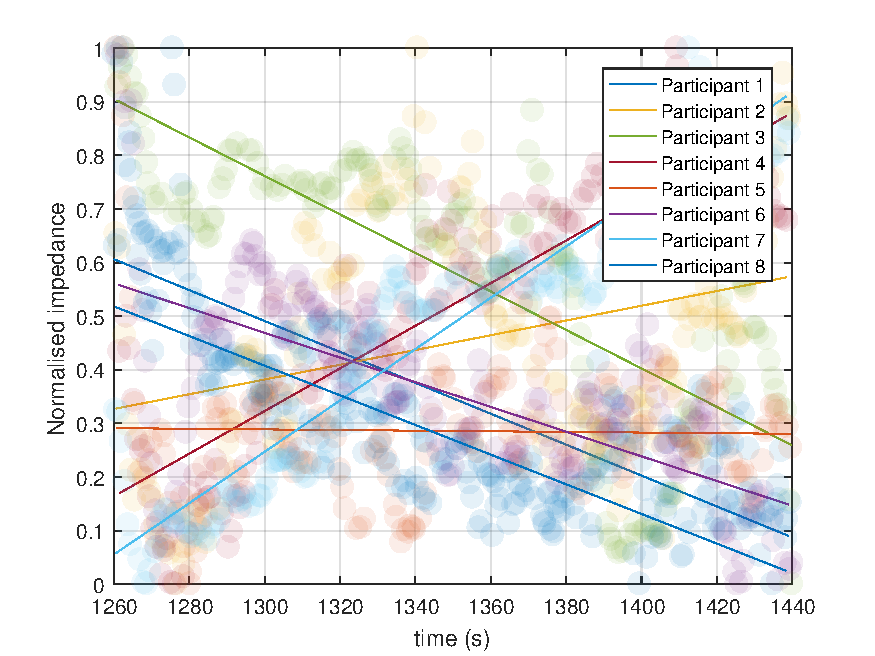
\includegraphics[width=0.65\textwidth,keepaspectratio]{figure5}    
	\caption[Doppler technique to measure flow]{Representation of the Doppler technique measuring blood flow. The cylinder represents the vessel; the red dots are the RBCs. The \textit{Ft} and \textit{Fr} are the frequencies of transmission and reception of the sensor. The phase shift between both signals change according to the movement of the particles.}
	\label{fig:Doppler method}
\end{figure}

Estimating blood flow based on this principle requires the measurement of arterial diameter and the blood velocity. Using these parameters, it becomes possible to calculate the blood flow by multiplying the blood's mean velocity (\si{\cm \per \second}) by the cross-sectional area of the artery in \si{\square \cm}, before multiplying it by \SI{60}{seconds} to express the value in millilitres per minute (\si{\milli\litre\per\minute}) \cite{casey2008measuring}. 

Some of its advantages include non-invasiveness, the ability to measure velocity continuously, portability (and hand-held), and less energy consumption, which makes it an excellent choice for home use. However, this method is not without its share of disadvantages. First, the operator requires some skill to be able to locate the artery accurately. Some instruments provide a sound feedback pertaining to the flow velocity of the artery. However, there are different levels of sound or pitch in order to identify the right vessel correctly. Second, it is recommended to use a low insonation angles ($\sim$ \SI{60}{\degree}) for limiting the number of errors \cite{raadegran1999limb} which also require steady hands from the operator. Third, it is effective when the limb and the artery remain in a fixed position; it is quite sensitive to motion. Lastly, as mentioned previously, it requires measuring the arterial diameter to convert velocity into flow, which marks a significant disadvantage because the only way to measure this parameter accurately is by making use of imaging methods \cite{chapter4bloodflow} but this could be quite an ardours task in a home setting.

\subsection{Optical methods measuring blood flow}
\label{section literature Optic}
Light is one of the most common electromagnetic energies applied on the field of medicine. Using optical methods makes it possible to estimate blood flow by measuring volume changes or by applying complex imaging techniques. One of the key features of this method is its mostly non-invasive or inclusive contact-less for some applications. Furthermore, optical imaging techniques are advantageous in that they offer a high resolution; they are also cost effective when compared to MRI or PET, apart from being a non-ionising source \cite{jayanthy2011measuring}.

It is one of the most popular methods to monitor continuously volume changes using the principle of optical absorption of the arterial blood. In principle, it requires a coherent light source provided by a laser/light emitting diode (LED) set to a specific wavelength in accordance to the application. The light propagates due to the transport of individual photons, which under the area of influence, may be absorbed or scattered \cite{schmitt2003quantitative}. 

This method is so popular that it is used in mostly every clinical setting as well as for personal use. The latter has become extensively available owing to the use of activity monitors that utilise optical methods, such as one employed in the Apple Watch \cite{culbert2017user}. This makes it clear that this method can be applied to home settings owing to its versatility and portability. The following application describes the methods to estimate the rate of flow. 

\subsubsection{Photoplesthymography}
\label{section literature PPG}
The word plethysmography owes its genesis to the Greek word \textit{plethysmos} which means an increase in population and \textit{graphos} that is to write. In other words, it can be defined as the measurement of any volume within the human body. In medicine, some of the typical applications include the measurement of volume changes in lungs caused by the respiratory system, or the blood vessels caused by the circulatory system~\cite{turcott2004methods}. More specifically, when referring to the latter, plethysmography aims to measure the pulsatile volume changes when the heart pumps blood in and out of a segment within the human body. 

A plethysmography device produces an output waveform that is synchronous to the heart cycle. The shape of the signal is similar to an arterial pressure waveform. In fact, the plethysmography plot represents the volume of the arterial vasculature that obtains a measure of the arterial pulse amplitude. This waveform gives key insights into the pulse velocity and indications of a possible arterial obstruction.

This method is technically known as photoelectric plethysmography, or PPG. Nowadays, it is one of the most popular methods in the parlance of medical applications. It is non-invasive and can accommodate a wide range of light wavelengths to obtain a plethysmography graph. It is widely used for the purpose of monitoring heart rate, oxygen saturation, peripheral arterial pressure and peripheral microcirculation after skin grafting, drug ingestion, burns or revascularization~\cite{holohan1996plethysmography}. There are two different techniques to obtain the readings. One is transmission-mode (see figure \ref{fig:PPG transmission}.) which works by placing the tissue of interest (i.e. finger, toe or ear lobe) between the light emitting diode (LED) and the photoreceptor (PD). The other is in the PPG reflectance-mode (see figure\ref{fig:PPG reflectance}) by placing the LED next to the photoelectric cell over the surface of the tissue. PPG leverages the AC component of the signal for arterial pulse detection and the DC component for venous evaluation~\cite{higgins1986photoplethysmographic}. It also uses different kinds of wavelengths to avoid interference from external sources of light. The underlying principle behind PPG detects the degree of attenuation of backscatter light from the superficial layers of skin about \SIrange{1.5}{2.0}{\milli\meter} ~\cite{holohan1996plethysmography,bashkatov2005optical,kim1986pulse}. The amount of reflected light varies in accordance with the total number of RBC's in the cutaneous micro-circulation, which alters the wavelength during each cardiac cycle. This method provides valuable insights based on the waveform analysis into the initial diagnostics of peripheral arterial disease (PAD) \cite{allen1993development, williams2005evaluation, alnaeb2007optical} and chronic peripheral venous insufficiency (CVI) \cite{eberhardt2005chronic,norris1983quantitative}.


\begin{figure*}[!htbp]
	\centering
	\begin{subfigure}[t]{0.45\textwidth}
		\centering
		\includegraphics[height=4cm]{figure7a}
		\caption{Placement of LED and photodetector in transmission mode}
		\label{fig:PPG transmission}
	\end{subfigure}%
	~ 
	\begin{subfigure}[t]{0.45\textwidth}
		\centering
		\includegraphics[height=4cm]{figure7b}
		\caption{Placement of LED and photodetector in reflectance mode}
		\label{fig:PPG reflectance}
	\end{subfigure}
	\caption[PPG sensors placemens as transmission and reflectance modes]{PPG light emitter placement and receptor according to the mode, transmission and reflectance}
	\label{fig:PPG modes}
\end{figure*}

It is plausible to conclude that plethysmography is not a stand-alone quantitative blood flow measurement, but an estimation of the blood concentration of a volume of tissue. While this assumption is not incorrect, studies have suggested that it is possible to estimate blood flow when combining optical methods with other techniques. For instance, using the tissue absorption of the near-infrared spectroscopy (NIRS) makes it possible to estimate blood flow, when combined with venous occlusion plethysmography (see section \ref{section literature VOP}) \cite{van2001performance, harel2008near, de1993noninvasive, gurley2012noninvasive}. NIRS takes the principle of the different levels of absorption of oxygenated and deoxygenated haemoglobin, thus forming the dynamic absorption pattern to determine the blood flow. The study performed by Gurley et al. demonstrates the increase of total haemoglobin concentrations (THC) during venous occlusion, which can be converted from \si{\micro M  \ tHB\per\sec} to \si{\mL \ blood \per 100 \ \mL \ tissue \per\min}.

One of the biggest disadvantages of PPG is that it only measures a small area at a given point in time. Therefore, it is not possible to get a spatial distribution of the blood volume change over a significant portion of the skin \cite{wu2003ppgi}. Additionally, skin pigmentation has proven to be a factor of error and nail polish \cite{fallow2013influence}. Also, light scattering in tissue makes it impossible to estimate its complete penetration in the skin. Therefore, it is not possible to calculate the volume of tissue being measured.


\subsubsection{Laser Doppler Flowmetry}
\label{section literature LDF}
LDF refers to a non-invasive optical method to estimate the blood perfusion within the microcirculatory bed under the skin. This device uses the same Doppler principle described in section \ref{section literature UD}. However, as the name suggests, it uses a beam of light as the electromagnetic source. It requires a laser diode emitting a wavelength commonly between \SI{633}{\nano\metre} (red) and \SI{780}{\nano\metre} (near-infrared) with an intensity of close to \SI{1}{\milli\watt} \cite{fredriksson2007laser}. A flexible fibre optic delivers and detects the light applied to a roughly \SI{1}{\cubic\mm} of tissue. Subsequently, the light scatters by tissue as well as the moving blood cells. Scattering by way of a moving blood cell with haemoglobin produces a frequency shift, whereas scattering from stationary tissue yields the opposite results. The velocity of the red blood cell passing through the beam is equivalent to the frequency shift. 

An analysis of the backscattered light provides crucial information on blood cell velocity given by the frequency of Doppler shift \cite{fredriksson2007laser,dirnagl1989continuous}, and the fraction of the backscattered light that is Doppler shifted is proportional to the total volume of moving blood cells concentrated within the tissue \cite{dirnagl1989continuous}. As a result, an index of red blood cells flow is calculated from the product of mean Doppler shift and the fraction of light that is Doppler shifted \cite{dirnagl1989continuous}. This blood perfusion index is also called flux. Figure \ref{fig:LDF method} overviews the laser doppler flowmetry theory, whereas additional details behind this principal are illustrated described in the works of Fredriksson et al. \cite{fredriksson2007laser}.  

\begin{figure}[!htpb]
	\centering
	\includegraphics[width=0.8\textwidth,keepaspectratio]{LDF}    
	\caption[Laser Doppler flowmetry theory overview]{The electromagnetic wave is emitted by light $E_L(t)$, the interaction with a red blood tissue produce backscatter light $\beta_L$. The photodetector detects the light and process the frequencies of the backscattered light that produces a power spectral density $P(\omega)$ that allows to estimate the concentration of moving blood cells (CMBC) and the perfusion index (\textit{Perf}). This image has been copied from \cite{fredriksson2007laser} to explain the theory behind LDF}
	\label{fig:LDF method}
\end{figure}

Some instruments can monitor blood flow in absolute blood flow units. However, some doubts persist about this quantification because the value is premised on an empirical calibration correlated to other methods \cite{cooke1990laser}. Another drawback is that the measurement is quite superficial; the penetration of the wavelength used by LDF is quite shallow. For instance, light in the wavelength of \SI{840}{\nano \metre} only penetrates up to \SI{2.5}{\milli\metre} \cite{bashkatov2005optical}, with the total volume of tissue being studies being quite small - at about \SI{0.1}{\cubic\mm} or less \cite{briers2013laser}. Therefore, location remains a key component in the context of obtaining a proper measurement as an area with a good amount of capillaries equals to a greater blood flow distribution around the surface of the skin. Thus, more blood particles can be detected without having to go deeper into the tissue. 

This method can be used within a home setting as well; it is portable, easy to locate and battery operated. Nonetheless, it does suffer from some shortcomings. Firstly, the measurement is affected by temperature in that it is recommended to have a stable room temperature. Secondly, it is vulnerable to motion artefact, and the probe must be attached firmly \cite{fredriksson2007laser}. 

\subsubsection{Laser speckle contrast imaging (LSCI)}
\label{section literature LSC}
The Laser speckle laser is a fairly new technique that is still being studied. Some medical applications under this method have measured cerebral blood flow \cite{dunn2001dynamic}, microcirculatory research \cite{domoki2012evaluation}, dentistry \cite{stoianovici2011assessment} and wound assessment \cite{stewart2005comparison} to name a few. This method can be catalogued as an imaging technique because it requires processing of images in order to obtain a coherent result. 

\begin{figure}[!htpb]
	\centering
	\includegraphics[width=0.8\textwidth,keepaspectratio]{lsci}    
	\caption[Setup of a Laser speckle contrast imaging]{A LSCI device requires a laser illuminating a surface, a CCD camera and a computer for the statistical analysis of the images. Image retrieved from \cite{son2013contrast}}
	\label{fig:LSCI}
\end{figure}


The set-up of a LSCI instrument is a fairly simple process, but the processing behind it can be quite complicated. Figure \ref{fig:LSCI} illustrates a common experimental procedure. A coherent (laser) light beam illuminates a sample recorded by a CCD (Charge Coupled Device) camera. A custom software captures the speckle pattern, which is then processed by a computer and displayed as an image \cite{jayanthy2011measuring, son2013contrast, duncan2008can}. The software controls the camera's exposure time, amount of pixels, local contrast area as well as the option of colours to code the contrast. 

Speckle images are generated by the interference pattern produced by the laser beam scattered on a rough surface, which is a random intensity distribution pattern created by the random refractive index fluctuations of the sample. This speckle pattern can only be explained by statistics \cite{goodman1975statistical}. As is the case with LDF, stationary tissue produces a constant intensity contrast; however, scattering from moving particles like blood cells produce fluctuations in the intensity of the speckle pattern \cite{son2013contrast}. These fluctuations end up reducing the local speckle contrast; hence the contrast value is inversely proportional to the blood flow speed. 

LCSI can be used within a home setting. Some of the advantages of the device are as follows: it is portable and can probably be battery operated if a mobile device replaces the computer. No exogenous material is required to produce a high spatial-temporal resolution image \cite{duncan2008can}, thus making it completely non-invasive. The image generated is easy to decipher even for non-experts. A technical improvement with Doppler techniques is that area is confined to the focal distance of the camera, whereas Doppler targets a single point measurement. However, there are some disadvantages of this method. For instance, the image is merely a representation of the surface vasculature; it is not possible to monitor the blood flow of large vessels. Although studies are being performed in order to quantify regional blood flow, this method continues to be a qualitative method until the statistics behind it are better-understood \cite{duncan2008can}. 

\subsection{Venous occlusion plethysmography}
\label{section literature VOP}
Venous occlusion plethysmography (VOP) is a common method used to assess different vascular problems in humans, particularly those that relate to the limbs. It has been around for more than 100 years, providing valuable insights into the behaviour and extent of the vascular endothelium in health and disease \cite{joyner2001belfast}. This method uses plethysmography to evaluate the patient's vascular response. However, estimating blood rate from this method requires it to be used in conjunction with instruments that are capable of measure the change of volume around a limb.

The principle behind VOP is that a pneumatic cuff is inflated around the upper-arm or tight below diastolic pressure, commonly about \SIrange{40}{50}{\mmHg}. Thus, the arterial inflow continues toward the limb even as the venous outflow is blocked \cite{casey2008measuring, joyner2001belfast}. As a result, the blood pooling effect swells the limb and raises its volume. The blood flow rate is then calculated as linear hikes of the limb's volume over time, which is believed to be proportional to the rate of arterial inflow \cite{casey2008measuring, joannides2006clinical}.

One could argue that having a cuff within a home setting could be cumbersome or may require some assistance. However, there have been recent developments in portable blood pressure monitors, which have greatly simplified this approach. For instance, as shown in figure \ref{fig:nokiabpm}, the Nokia BPM+ \cite{nokiabpm} is a wireless instrument that automates the process of obstructing the upper arm.

\begin{figure}[!htpb]
	\centering
	\includegraphics[width=0.65\textwidth,keepaspectratio]{nokiabpm}    
	\caption[Nokia BPM+]{Portable blood pressure monitor from Nokia. Image retrieved from \cite{nokiabpm}}
	\label{fig:nokiabpm}
\end{figure}

Apart from the cuff, it is important to measure plethysmographic changes around the limb in order to estimate blood flow. To that end, a gamut of instruments has been used within a clinical setting to estimate the rate of flow, although only a few have the potential of being used at home. The following are some of the currently available methods.  

\subsubsection{Air/Water plethysmography}
\label{section literature air plethysmography}
Air/water plethysmography is not a common method that us used to measure a limb's change of volume. Its efficacy is primarily that of an alternative research method, as explained by Chuah et al.~\cite{chuah2004plethysmography} for measuring plethysmography without venous occlusion. This approach uses a special chamber that contains the limb within a closed area with orifices where transducers and calibration devices are connected. The arm is introduced into the case using a tight rubber sleeve to ensure that the instrument is airtight.  The plethysmography pulsations are detected by measuring the displacement of the surrounding air with a sensor connected to the chamber; this also moves the rubber diaphragm whereby a Doppler ultrasound transducer measures the extent of displacement. 

This method can provide fairly accurate results, but motion artefact does cause some ripples movements that affect the final value. Furthermore, this method could be burdensome in a home setting, or even for surgery applications. It requires an extra participant to aid arm positioning within the chamber and perform the adequate calibration. Also, the portability of this method is quite questionable and requires a number of parts to work simultenously.

\begin{figure}[!htpb]
	\centering
	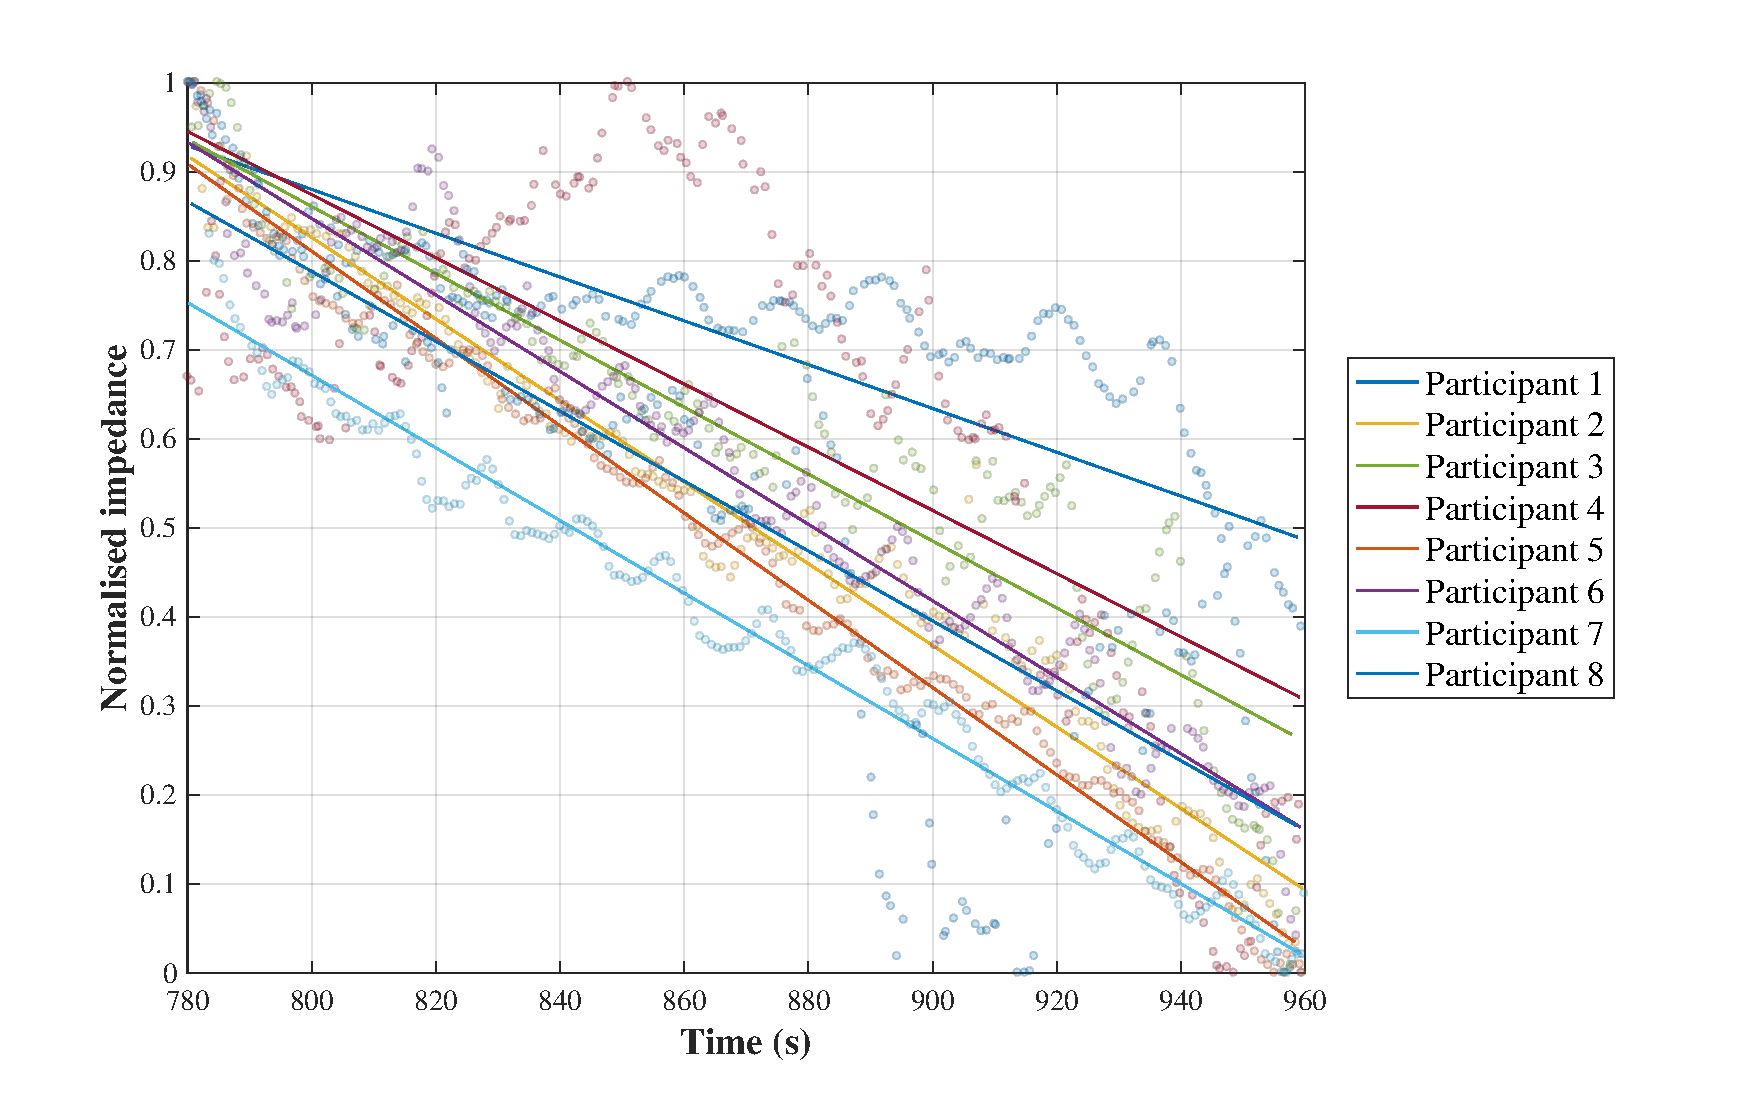
\includegraphics[width=0.8\textwidth,keepaspectratio]{figure4}    
	\caption[Air plethysmography method]{Representation of an air plethysmography device. It requires a one-side open cylinder with a rubber sleeve. There is a compartment where the air displacement caused by each cardiac cycle can be measured. Image reproduces from \cite{chuah2004plethysmography}}
	\label{fig:air plethysmography}
\end{figure}

\subsubsection{Strain gauge plethysmography}
\label{section literature stain grauge}
This method also known as SGP (strain gauge plethysmography), and is a non-invasive method to quantify retrograde outflow in the deep venous system and peripheral arterial disease \cite{holohan1996plethysmography}. It works by applying a strain gauge around the limb being studied. The transducer could be a tube filled in with a conductive material, such as mercury and gallium, and is connected to a source of electricity. However, alternative methods that do not use clinically banned mercury have been developed using electrical conductive fluids \cite{flowers1981strain}. When the gauge experiences variations of circumference triggered by a change in volume of the rib cage or the pulse in a limb, the resistance of the sensor varies accordingly, thus obtaining an electrical waveform. Increasing the sensitivity for venous filling measurements requires occlusion cuffs, as shown in Figure~\ref{fig:strain gauge}. This method does not provide reliable quantitative data for venous occlusion, although it does offer qualitative data for the function of the extremity in venous insufficiency \cite{holohan1996plethysmography}. 

This method presents some advantages when used within a home setting. First, it is portable since only a single point of measurement is required. Second, it is non-invasive, and requires minimal skills. However, one latent problem is the use of mercury on some sensors; it is a poisonous metal and is not recommended to be used at home. New electrodes can be used \cite{flowers1981strain} instead. Moreover, the instrument merely measures changes of volume in a confined circumference around the sensor. In other words, it does sense changes around a large volume of tissue. 

\begin{figure}[!htpb]
	\centering
	\includegraphics[width=0.75\textwidth,keepaspectratio,trim={0.5cm 0.5cm 0.5cm 0.5cm}, clip]{figure6}    
	\caption[Strain gauge plethysmography]{Representation of a classic plethysmography waveform from the heart cycle. The image on the top represents the electrical signal of the heart. The one before it is the plethysmography waveform of the circulation.}
	\label{fig:strain gauge}
\end{figure}

\subsubsection{Bioelectrical Impedance plethysmography}
\label{section literature BI}
Bioelectrical impedance plethysmography is yet another method that measures changes in blood volume in different parts of the body, such as the thoracic cavity or limbs \cite{bera2014bioelectrical}. In principle, it senses small changes of bioelectrical impedance due to the increase of blood cells in a volume of tissue. For instance, when the heart's systole increases the blood flow, the volume of a limb rises in accordance with the inflow of blood (swelling) \cite{martinsen2011bioimpedance}. Consequently, the changes of impedance are correlated to the small variation of volume and flow in a limb. Some medical applications might necessity the use of pneumatic cuffs in order to analyse venous filling. There are several medical applications for this kind of technique, such as heart stroke volume (SV) measurement, cardiac output (CO), thoracic respiratory volume, oedema and the detection of deep vein thrombosis (DVT) \cite{holohan1996plethysmography}. 

Bioelectrical impedance plethysmography has been demonstrated to have a linear relation with other plethysmographic instruments, like strain gauge. For instance, the studies carried out by Mohapatra~\cite{mohapatra1979measurement} and Schraibman~\cite{schraibman1975comparison} revealed a significant relationship between both techniques.

In the chapter \ref{chapter impedance} the principles of operation of this technology are described in greater detail. In summation, this method requires the application of a small amount of current into the body at a specific frequency and amplitude, usually between \SIrange{1}{500}{\kHz} \cite{kyle2004bioelectrical} and bellow \SI{5}{\mA}. The body's bioelectrical impedance is a relation between the electrical potential and the electrical current (applied). Commonly, a set of four electrodes is placed atop the surface of the skin where a pair converts the electrical conductivity into ionic conductivity to sense the voltage drop. An increase in the amount of blood within a section of body drops its total impedance. Therefore, there is a direct correlation between the population of red blood cells and the measurement of impedance \cite{mattern1957determination}. 

The blood flow rate can be estimated from the impedance plethysmography signal. Indeed, impedance maybe regarded as a measurement of both volume and flow; a change of volume must be attributed to a flow \cite{martinsen2011bioimpedance}. Some studies incorporate venous occlusion plethysmography as a method to estimate the flow rate \cite{mohapatra1979measurement, costeloe1980continuous, yamakoshi1980limb}, whereas other techniques focus on the analysis of the plethysmographic signal without integrating occlusion \cite{porter1985measurement,corciova2011peripheral, brown1975impedance, marks1985computer}. 

Nyober et al. \cite{nyober1950electrical} proposed the reigning equation \ref{eq:DVDT} from which, the blood flow is estimated. The author opined that the the blood flow is proportional to the change of impedance in relation to the distance between the potential electrodes and basal impedance of the tissue. The section \ref{section procedure Z to V and Q} describes the equation required to convert impedance into the blood flow in greater detail.

Calculating blood flow from the impedance signal is applicable in home settings as well. Being non-invasive, it only requires four electrodes for measurement, which is one of its main advantages. Additionally, the device uses low-energy in that the current required to read impedance is below \SI{5}{\mA} which can be obtained from a battery operated instrument. Furthermore, the tissue's volume being monitored is more substantial as compared to other techniques, given that the boundary of this measurement is limited by the position of potential electrodes. In fact, the body measurements can be  attained as described in free-fat measurements undertaken by Kyle et al. \cite{kyle2004bioelectrical}. IPG is less affected by temperature \cite{bera2014bioelectrical}; furthermore, it provides more data than single point measurements to better assess venous blood volume and arterial pulsations \cite{bera2014bioelectrical}. However, this technique does have some shortcomings as well.   Like all the methods, it is also sensitive to motion. Secondly, electric current is required for undertaking a measurement, which makes is unsuitable for a certain category of population. Finally, there is an electrode-skin impedance error in the absence fo a full contact. 

\section{Conclusion}
This section introduced the circulatory system beginning from blood cells and its functionality. It is important to reiterate the importance of blood cells in transporting nutrients and oxygen whole tissue around the body. The blood vessels structure was explained and more light was shed on the manner in which blood reaches every cell in the body, along with an interchange of nutrients and by-products. The cardiac cycle demonstrated exactly how heart operates as a pump and how blood flows in and out of it. The anatomy of the upper extremities will serve as a reference when advancing further in this document.  

Illnesses and problems caused by poor circulation towards the periphery were also described, along with an explanation of the rationale behind monitoring blood flow in a home setting. Subsequently, different instruments were elaborated upon, along with the potential to quantify blood flow in a home environment. In addition, the Doppler Ultrasound method was described along with the various optical instruments. The venous occlusion plethysmography is a useful tool for quantifying blood rate. Three different apparatuses have the potential of being used at home. However, obtaining the flow rate from the bioelectrical impedance plethysmography seems to be an excellent choice because it is able to assess a larger volume of tissue as compared to other methods.


%********************************** %Nomenclatures in chapter  **************************************
\nomenclature[z-Hb]{Hb}{Haemoglobin}
\nomenclature[z-ATP]{ATP}{Adenosine Triphosphate}
\nomenclature[z-rbc]{RBC}{Red Blood Cells}
\nomenclature[z-abi]{ABI}{Ankle-Brachial index}
\nomenclature[z-wbc]{WBC}{White Blood Cells}
\nomenclature[z-PVD]{PVD}{Peripheral vascular disease}
\nomenclature[z-bia]{BIA}{Bioelectrical impedance analysis}
\nomenclature[z-DFI]{DFI}{Doppler flowmetry}
\nomenclature[z-DVT]{DVT}{Deep vein thrombosis}
\nomenclature[z-cli]{CLI}{Critical Limb Ischemia}
\nomenclature[z-PAD]{PAD}{Peripheral Arterial Disease}
\nomenclature[z-SV]{SV}{Strove Volume}
\nomenclature[z-LED]{LED}{Light emitting diode}
\nomenclature[z-CVI]{CVI}{Chronic peripheral venous insufficiency}
\nomenclature[z-ppg]{PPG}{Photoplethysmography}
\nomenclature[z-ipg]{iPG}{Impedance Plethysmography}
\nomenclature[z-CO]{CO}{Cardiac output}
\nomenclature[z-SGP]{SGP}{strain gauge plethysmography}
\nomenclature[z-BIA]{BIA}{Bioelectrical impedance analysis}
\nomenclature[z-NIRS]{NIRS}{Near-infrared spectroscopy}
\nomenclature[z-LSCI]{LSCI}{Laser speckle contrast imaging}
\nomenclature[z-CCD]{CCD}{Charge Coupled Device}


%\nomenclature[z-cif]{$CIF$}{Cauchy's Integral Formula}                                % first letter Z is for Acronyms 
%\nomenclature[a-F]{$F$}{complex function}                                                   % first letter A is for Roman symbols
%\nomenclature[g-p]{$\pi$}{ $\simeq 3.14\ldots$}                                             % first letter G is for Greek Symbols
%\nomenclature[g-i]{$\iota$}{unit imaginary number $\sqrt{-1}$}                      % first letter G is for Greek Symbols
%\nomenclature[g-g]{$\gamma$}{a simply closed curve on a complex plane}  % first letter G is for Greek Symbols
%\nomenclature[x-i]{$\oint_\gamma$}{integration around a curve $\gamma$} % first letter X is for Other Symbols
%\nomenclature[r-j]{$j$}{superscript index}                                                       % first letter R is for superscripts
%\nomenclature[s-0]{$0$}{subscript index}                                                        % first letter S is for subscriptsd
